\documentclass[12pt]{article}
\usepackage[top=1in, bottom=1in, left=.75in, right=.75in]{geometry}
\usepackage{amsmath}

%WATER MARK OPTION
%\usepackage{draftwatermark}
%\SetWatermarkText{draft}
%\SetWatermarkScale{1}
%\SetWatermarkLightness{.9}

%\usepackage[]{enumitem}
\usepackage{enumerate}
\usepackage{fancyhdr}
\usepackage{graphicx, xcolor, setspace, adjustbox}
\usepackage{txfonts}
\usepackage{multicol,coordsys,pgfplots}
\usepackage[scaled=0.86]{helvet}
\renewcommand{\emph}[1]{\textsf{\textbf{#1}}}
\usepackage{anyfontsize}
% \usepackage{times}
% \usepackage[lf]{MinionPro}
\usepackage{tikz,pgfplots}
%\def\degC{{}^\circ{\rm C}}
\def\ra{\rightarrow}
\usetikzlibrary{calc,arrows.meta, shapes, angles, quotes}
\pgfplotsset{compat = newest}
\newcommand{\blank}[1]{\rule{#1}{0.75pt}}

\pgfplotsset{my style/.append style={axis x line=middle, axis y line=
middle, xlabel={$x$}, ylabel={$y$}}}


%\usepackage{draftwatermark}
%\SetWatermarkText{Draft}
%\DraftwatermarkOptions{color={[gray]{.9}}}
%\SetWatermarkScale{1.5}

%axis equal

%yticklabels={,,} , xticklabels={,,}

% \setmainfont{Times}
% \def\sansfont{Lucida Grande Bold}
\parindent 0pt
\parskip 4pt
\pagestyle{fancy}
\fancyfoot[C]{\emph{\thepage}}
\fancyfoot[R]{v1}
\fancyhead[L]{\ifnum \value{page} > 1\relax\emph{Math F251X Calculus I: Final Exam}\fi}
\fancyhead[R]{\ifnum \value{page} > 1\relax\emph{Fall 2024}\fi}
\headheight 15pt
\renewcommand{\headrulewidth}{0pt}
\renewcommand{\footrulewidth}{0pt}
\let\ds\displaystyle
\def\continued{{\emph {Continued....}}}
\def\continuing{{\emph {Problem \arabic{probcount} continued....}}\par\vskip 4pt}


\newcounter{probcount}
\newcounter{subprobcount}
\newcounter{subsubprobcount}
\newcommand{\thesubproblem}{\emph{\alph{subprobcount}.}}
\newcommand{\thesubsubproblem}{\emph{\roman{subsubprobcount}.}}
\def\problem#1{\setcounter{subprobcount}{0}%
\addtocounter{probcount}{1}{\emph{\arabic{probcount}.\hskip 1em(#1)}}\par}
\def\subproblem#1{\par\hangindent=1em\hangafter=0{%
\addtocounter{subprobcount}{1}\thesubproblem\emph{#1}\hskip 1em}}
\def\subsubproblem#1{\par\hangindent=1em\hangafter=0{%
\addtocounter{subsubprobcount}{1}\thesubsubproblem\emph{#1}\hskip 1em}}
\def\probskip{\vskip 10pt}
\def\medprobskip{\vskip 2in}
\def\subprobskip{\vskip 45pt}
\def\bigprobskip{\vskip 4in}


\newenvironment{subproblems}{%
\begin{enumerate}%
\setcounter{enumi}{\value{subprobcount}}%
\renewcommand{\theenumi}{\emph{\alph{enumi}}}}%
{\setcounter{subprobcount}{\value{enumi}}\end{enumerate}}

\newenvironment{subsubproblems}{%
\begin{enumerate}%
\setcounter{enumi}{\value{subsubprobcount}}%
\renewcommand{\theenumi}{\emph{\roman{enumi}}}}%
{\setcounter{subprobcount}{\value{enumi}}\end{enumerate}}


\newcommand{\be}{\begin{enumerate}}
\newcommand{\ee}{\end{enumerate}}


\begin{document}

{\emph{\fontsize{26}{28}\selectfont Fall 2024 \hfill
\hfill Math F251X}}

\begin{center}
{\emph{\fontsize{32}{36}\selectfont Calculus I: Final Exam}}
\end{center}
\vskip 1.cm

\strut\vtop{\halign{\emph#\hskip 0.5em\hfil&#\hbox to 2in{\hrulefill}\cr
\emph{\fontsize{18}{22}\selectfont Name:}&\cr
\noalign{\vskip 10pt}
%\emph{\fontsize{18}{22}\selectfont Student Id:}&\cr
%\noalign{\vskip 10pt}
%\emph{\fontsize{18}{22}\selectfont Calculator Model:}&\cr
}}
\hfill
\vtop{\halign{\emph{\fontsize{18}{22}\selectfont #}\hfil& \emph{\fontsize{18}{22}\selectfont\hskip 0.5ex $\square$ #}\hfil\cr
Section: & 9:15 (James Gossell)\cr
\noalign{\vskip 4pt}
         & 11:45 (Jill Faudree)\cr
\noalign{\vskip 4pt}
         & 11:45 (Leah Berman)\cr
\noalign{\vskip 4pt}
         & Online (James Gossell)\cr}}
%
%\vfill


{\fontsize{16}{18}\selectfont\emph{Rules:}}
\begin{itemize}
\item Partial credit will be awarded, but you must {\bf show your work}.

\item You may have a single handwritten $3'' \times 5''$ notecard, both sides.

\item Calculators are \emph{not allowed}. 

\item Place a box around your  \fbox{FINAL ANSWER} to each question where appropriate.

\item Turn off anything that might go beep during the exam.

\item You have two hours to complete the exam.

\end{itemize}

\def\emptybox{\hbox to 2em{\vrule height 16pt depth 8pt width 0pt\hfil}}
\def\tline{\noalign{\hrule}}
\centerline{\vbox{\offinterlineskip
{
\bf\sf\fontsize{18pt}{22pt}\selectfont
\hrule
\halign{
\vrule#&\strut\quad\hfil#\hfil\quad&\vrule#&\quad\hfil#\hfil\quad
&\vrule#&\quad\hfil#\hfil\quad&\vrule#\cr
height 3pt&\omit&&\omit&&\omit&\cr
&Problem&&Possible&&Score&\cr\tline
height 3pt&\omit&&\omit&&\omit&\cr
&1&&10&&\emptybox&\cr\tline
&2&&6&&\emptybox&\cr\tline
&3&&16&&\emptybox&\cr\tline
&4&&6&&\emptybox&\cr\tline
&5&&8&&\emptybox&\cr\tline
&6&&9&&\emptybox&\cr\tline
&7&&11&&\emptybox&\cr\tline
&8&&9&&\emptybox&\cr\tline
&9&&16&&\emptybox&\cr\tline 
&10&&9&&\emptybox&\cr\tline 
%&11&&?&&\emptybox&\cr\tline \tline 
&Extra Credit&&(5)&&\emptybox&\cr\tline \hline
&Total&&100&&\emptybox&\cr
}\hrule}}}

\newpage

%%%%%%%%%%%%%%%%% Compute some integrals
\problem{10 points} Compute the following \emph{integrals}. Give the most general answer, and show your work. Clearly indicate any substitutions you use in such a way that someone else can follow your work.

\begin{subproblems}
\item  $\ds \int \left(5t^{\frac{2}{7}} - 7t^{-1} + e^{3t-4} + \sin\left(\frac{\pi}{6}\right) \right)\: dt$
	\vfill
	\item $\ds \int x \cos(x^{2}) + \frac{1}{\sqrt{1-x^{2}}}  \: dx$
	\vfill 

\end{subproblems}

%%%%%%%%% Linearization
\problem{6 points}
Use linearization to estimate $\sqrt{98}$. Show your work, and write your answer as a single decimal or fraction.
	\vspace{2.5in}
	\newpage


%%%%%%%%% Miscellany of Questions about a given graph
\problem{16 points} Consider the graph of the function $f(x)$ shown below, and answer the following questions. You must give the most complete answer; if the value is infinite, write $+ \infty$ or $-\infty.$
	\vspace{-.5cm}
	\begin{center}
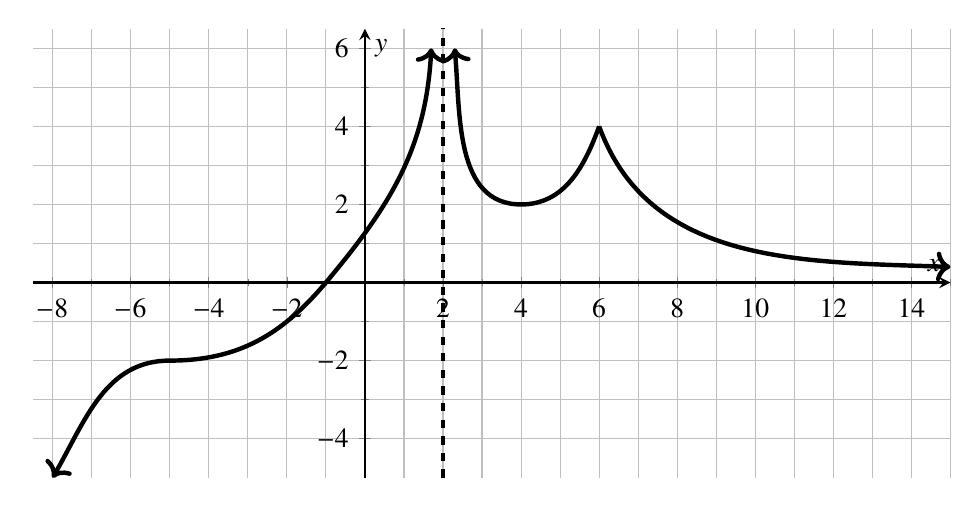
\begin{tikzpicture}[]
%cubic
\begin{axis}[%xscale = 1, yscale = 1, 
scale = 1.7,
axis equal image,
thick, my style, xtick={-8,-6,...,15}, ytick={-4,-2,..., 6},xmin=-8.5, xmax=15, ymin=-5, ymax=6.5, minor y tick num=1, minor x tick num=1, 
mark size=3.0pt, grid = both, ]
%\addplot[ultra thick, -,domain=-4:-2, samples=100, <-]coordinates {(-4,-2)(-2,2)};
%\addplot[ultra thick, domain=-5:-0.1, smooth] coordinates{(-3, -2) (0,0) (1.7, 5)(1.8, 6)};
\draw[ultra thick, <->](-8, -5) to[out = 60, in = 180] (-5, -2) to[out = 0, in = 180+50] (-1,0) to[out = 50, in = -93] (1.7,6);
%{sqrt(25-x^2)};
\draw[ultra thick, <-](2.3, 6) to[out = -85, in = 180] (4, 2) to[out = 0, in = -90-20] (6, 4);
\draw[ultra thick, ->](6, 4) to[out = -90+20, in = 180-2] (15, .4);
\draw[ultra thick, dashed] (2, -5) -- (2, 8);

%\addplot[ultra thick, ->,domain=5:9, samples=100]{-1/2*(x-5)};
\end{axis}


\end{tikzpicture}
\end{center}



\begin{subproblems}
\begin{multicols}{3}
\item $\ds \lim_{x \to 2^{-}} f(x) =$ \blank{1 cm}
\item $\ds \lim_{x \to 6} f(x) =$ \blank{1 cm}
\item $\ds \lim_{x \to 2^{+}} f'(x) =$ \blank{1 cm}
\end{multicols}
\item List all $x$-values where the derivative $f'(x)$ is not defined. 
\hrulefill
\item Estimate $f'(8)=$\blank{1cm}. \textbf{Explain} how you computed your estimate.

\vspace{1in}

\item List all intervals where $f'(x) >0$. \hrulefill
\item As what $x$-values does $f(x)$ have...(If none write ``none'').

 A local maximum? \hrulefill A local minimum? \hrulefill. 
 \item The line $y = 0$ is a horizontal asymptote of $f(x)$. Fill in a statement about a limit that corresponds to this fact.
 
\[\lim_{\fbox{\strut\hspace{1cm}}} \fbox{\strut\hspace{1cm}} = \fbox{\strut\hspace{1cm}}\]

 
 \item Does $f$ have an(y) inflection point(s)? If so, list it/them, if not write ``none.''
 
 Inflection point(s): $x = $ \blank{1.5 cm}
 
\item On what interval(s) is $f(x)$ concave down? \hrulefill
 \end{subproblems}

\newpage
%%%%%%%%%%%%%%%Part II of Miscellany of questions. Focused on FTC

\problem{6 points}
The graph of a function $g(x)$ is shown below.
\begin{center}
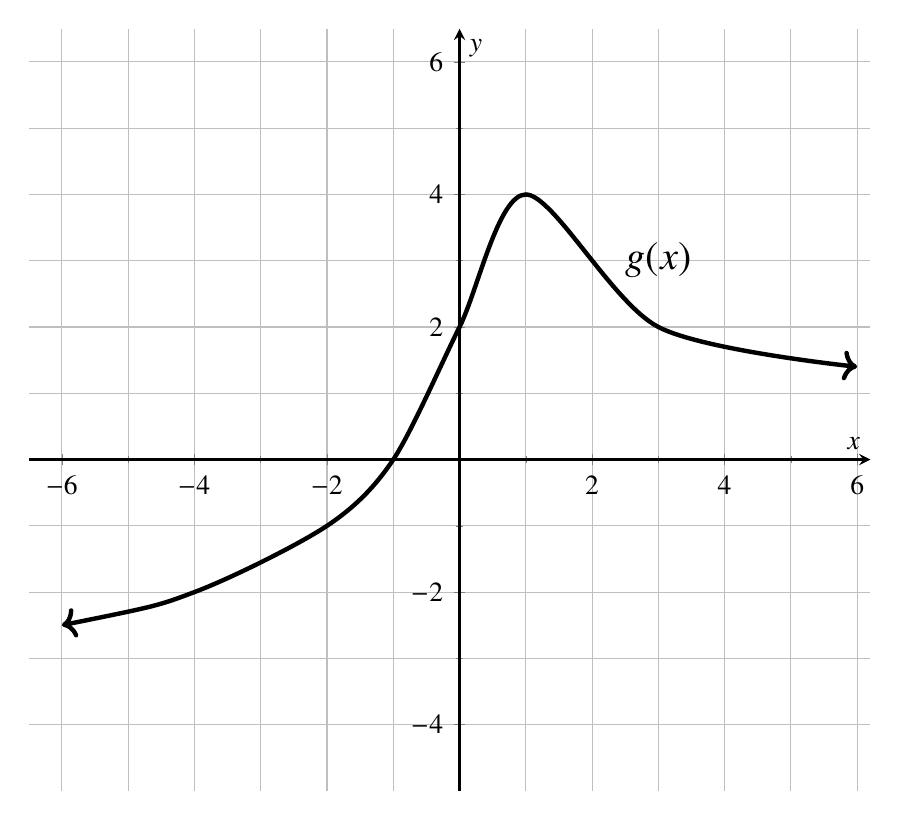
\begin{tikzpicture}[]
%cubic
\begin{axis}[%xscale = 1, yscale = 1, 
scale = 1.7,
axis equal image,
thick, my style, xtick={-8,-6,...,8}, ytick={-4,-2,..., 6},
xmin=-6.5, xmax=6.2, ymin=-5, ymax=6.5, minor y tick num=1, minor x tick num=1, 
mark size=3.0pt, grid = both, ]
\addplot[ultra thick, domain = -5:8, smooth, <->] coordinates{%(-8,-3)
(-6, -2.5)
(-4,-2)%(-3,-1.5)
(-2,-1)(-1,0)(0,2)%(1,3)
(1,4)(3,2)%(4,1.5)
(6,1.4)
%(8,1)
};
\path (3,3) node{{\Large $g(x)$}};

\end{axis}


\end{tikzpicture}
\end{center}

Define a new function $\ds A(x) = \int_{-4}^{x} g(t) \ dt$.
\begin{subproblems}
\item  On the interval $(-4, 4)$, does $A(x)$ have a local maximum or a local minimum? If so, give the corresponding $x$-value and \emph{explain} your answer. If not, explain why not.

\vfill

\item \emph{Estimate} %$\ds \int_{-5}^{1} f(x) \ dx$ = 
$A(0) = $\blank{1cm} and clearly explain what calculation you did to arrive at that estimation. (You may want to draw on the graph as part of your explanation.)

\vfill

\item Determine $A'(3) = $ \blank{1 cm}.

\end{subproblems}

\newpage
%%%%%%%%%%%%%%%%% Implicit Differentiation
\problem{8 points} 
Below is the graph of the curve $x^4+y^4+2x^2y=21.$
	
	\begin{subproblems}
	\item Find $\ds \frac{dy}{dx}$ for the curve $x^4+y^4+2x^2y=21.$
\hfill	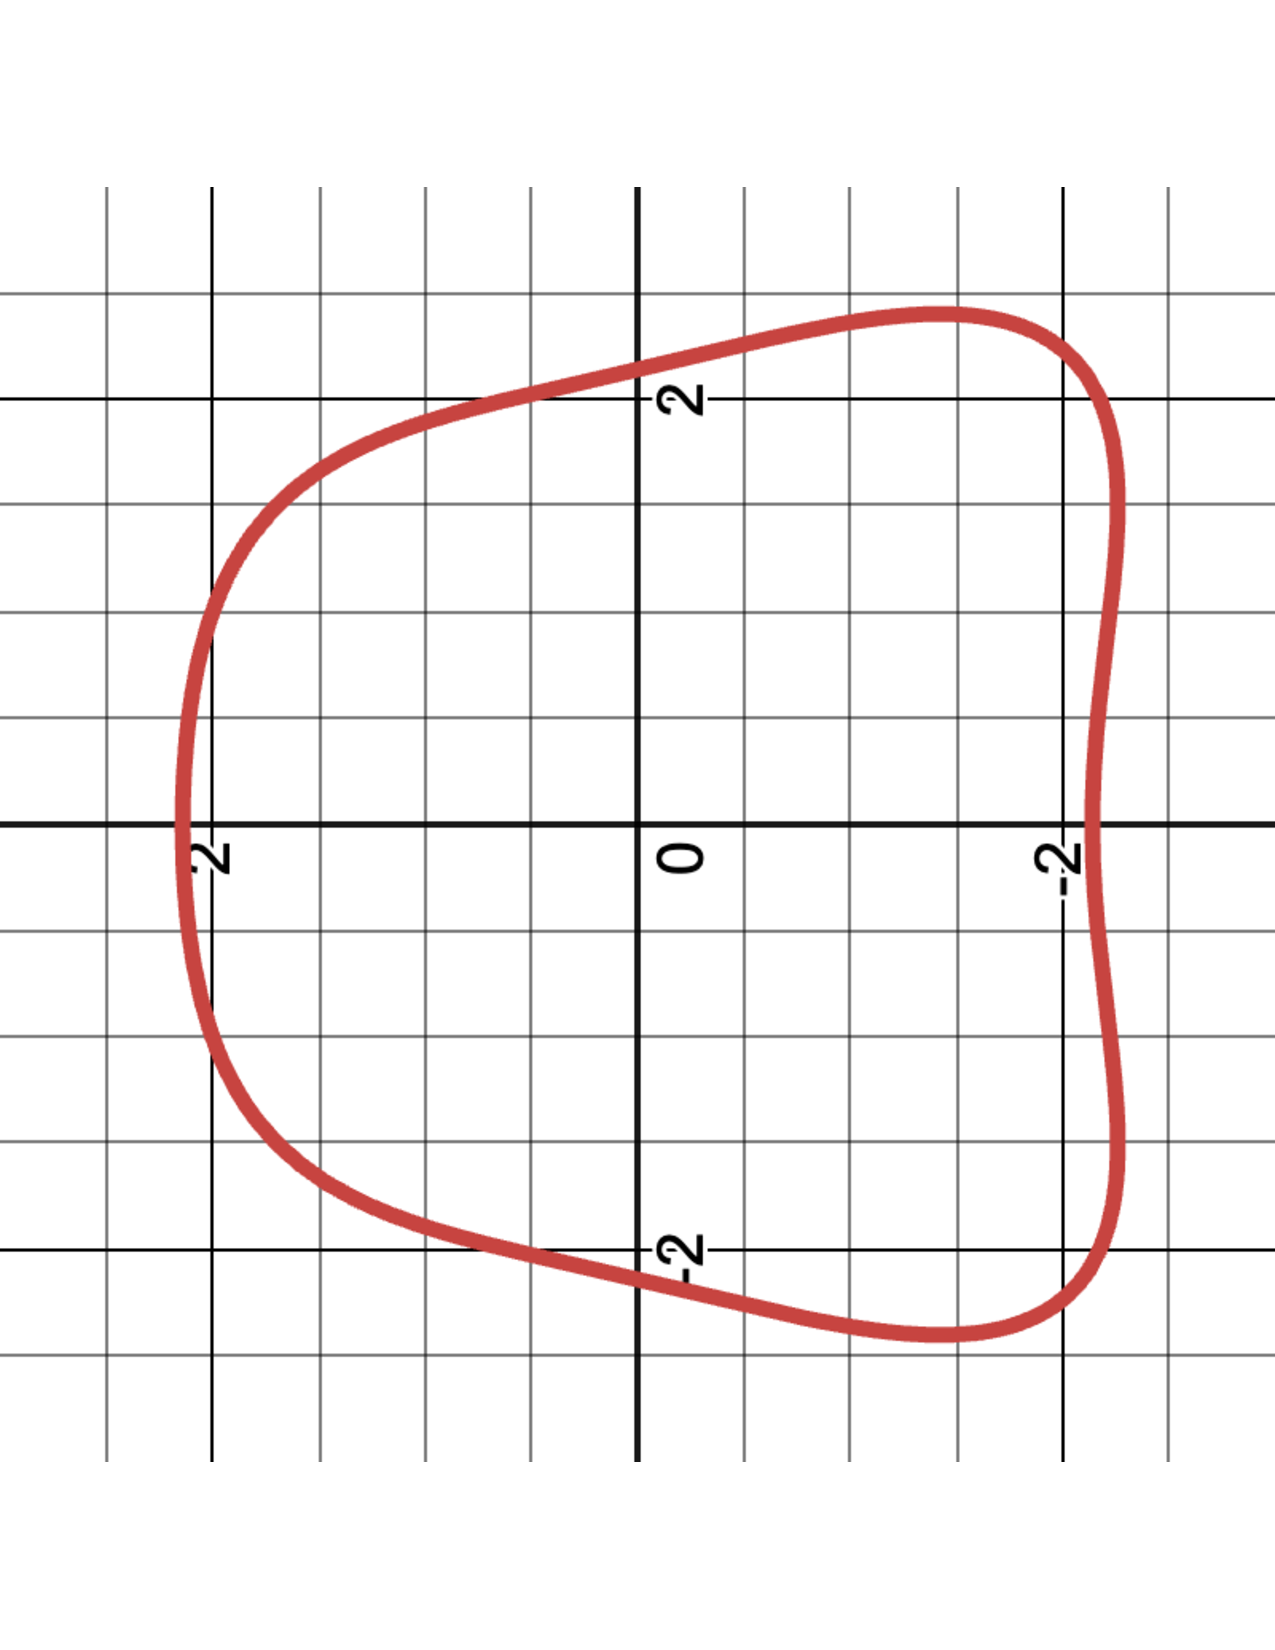
\includegraphics[scale=.25, angle=-90]{mid2-implicit-pic.pdf}
	\vfill

	\item \emph{Write an equation} of the line tangent to the curve $x^4+y^4+2x^2y=21$ at the point $(1,2)$. %\textcolor{red}{Version by using the point $(-1,2)$.}
	\vfill
	Tangent line equation: \hrulefill
	\item  \emph{Draw} the tangent line on the figure above.
	\end{subproblems}
	
\newpage	
%%%%%%%%%%%%%%%IVP + position, velocity, acceleration

\problem{9 points}  The Mars rover drops a rock off of a $61$ foot cliff. While in free fall, the rock's \emph{velocity} after $t$ seconds is given by the function $v(t) = -12.2t$ feet per second.
\begin{subproblems}
	\item Evaluate the integral $\ds \int_0^2 v(t) \: dt$ and write a sentence to interpret its meaning in the context of the problem. Include units in your answer.
	\vfill
	\vfill
	\item Write a function $h(t)$ that gives the rock's height above the ground after $t$ seconds.\\ %(Note that $h(0)=61$ since the rock starts $61$ feet above the ground.) 
	\vfill
	\item What is the \emph{acceleration} due to gravity on Mars? Include units in your answer.
	\vfill

	\end{subproblems}
\newpage

%%%%%%%%%%%%%%%%%%%% OPTIMIZATION
\problem{11 points} 

A box has a square base and an open top. The material for the base costs \$4 per square meter and the material for the sides costs \$1 per square meter. Suppose the width of the base of the box is $x$ meters and its height is $y$ meters.

	\begin{subproblems}
	\item What is the total cost, $C$, of the box?
	\vspace{.5in}
	\item What is the volume, $V$, of the box?
	\vspace{.5in}
	
	\item Suppose you have \$36 %(version 2 will use \$2700) 
	to spend on the materials for the box. 
		\begin{enumerate}[(i)]
		\item Write the volume $V$ as a function of one variable and pick a \emph{domain} for this function.
	\vspace{3cm}
		
		\item Determine the \emph{dimensions} of the box of \emph{largest} possible volume that fits within your budget. 
		\vfill
		\vfill
		dimensions (include units): $x = $ \blank{3cm} $y = $ \blank{3cm}
		\item \emph{Justify} that your dimensions give the largest volume,  using calculus. As part of your justification, \emph{write the name} of the test you are applying (first derivative test, second derivative test, closed interval/extreme value theorem, some other test).
		\vspace{3cm}
		\end{enumerate}
\end{subproblems}
	
\newpage

\problem{9 points} Compute the following \emph{limits}. Show your work clearly. Make sure you use \emph{limit notation} where required; an answer that does not use proper notation will not receive full credit. Use = to show things are equal. If you use L'H\^opital's rule, write $\stackrel{H}{=}$ or  $\stackrel{L'H}{=}$ to indicate where you are applying it.

\begin{subproblems}
\item $\ds \lim_{h \to 0} \frac{\ln(e+h)-1}{h}$
	\vfill
	\item $\ds \lim_{\theta \to \pi} \frac{\sin^2(\theta)}{1 + \cos(\theta)}$
	\vfill

	\item $\ds \lim_{x \to \infty} \frac{-8x^3 +5x^2}{2x^3 +3x - 5}$
	\vfill

\end{subproblems}

\newpage

%%%%%%%%%%%%%%%%% Net Change + Max Rate of Change
\problem{16 points} At 3:00 pm ($t = 0$), workers discover a break in an oil pipeline. The rate at which oil is flowing from the break is given by $\ds r(t)=\frac{10t}{4+t^2}$, where $r$ is measured in gallons per hour and $t$ is measured in hours.% from $t=0$ to $t=24.$
	\begin{subproblems}
	\item Find $r(1)$. Write a sentence that someone who has not taken calculus could understand to explain the meaning of $r(1)$. Include units.
	\vfill
	\item Determine how much oil flowed out of the pipeline between 3:00pm and 5:00pm. Include units in your answer.
	\vfill
	\item  At 4:00pm, is the rate of flow increasing, decreasing or staying the same? Explain how you know.%Show work and explain your answer. 
	
\vfill
	\item At what time is the rate of flow of the oil at its maximum? (Give your answer as a time.) %Show some work, and answer the question with a sentence.
	\vfill
	\end{subproblems}

\newpage

\problem{9 points} Compute the following \emph{derivatives}. Show your work. You do NOT need to simplify your answer. Your answer should start $f'(x)$, $\frac{df}{dx}$ etc.

\begin{subproblems}

\item  $\ds f(x)=x^{-4}+\sqrt[4]{(2x)}-4^x+4$
	\vfill
	\item $\ds g(x)=\ln\left(\frac{x^5e^x}{\sqrt{x}}\right)$
	\vfill
	\item $\ds h(x)=5\sec\left(2x^{-3}\right)$ %changed from arctan
	\vfill

\end{subproblems}

\newpage

%% Extra Credit Newton's Method
\fbox{\emph{Extra Credit}} (5 points) A portion of the graph of the function $f(x)=x - 5 \arctan(x)$ is shown below.

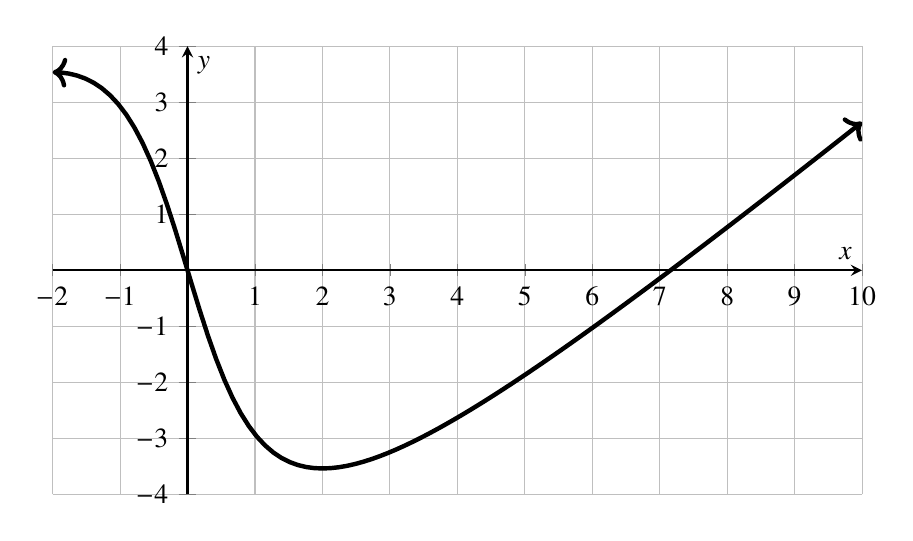
\begin{tikzpicture}[]
%cubic
\begin{axis}[%xscale = 1, yscale = 1, 
yscale = 1, xscale = 1.5,
%axis equal image,
thick, my style, xtick={-6,...,10}, ytick={-4,...,4},
xmin=-2, xmax=10, 
ymin=-4, ymax=4, 
minor y tick num=0, minor x tick num=0, 
mark size=3.0pt, grid = both, ]
%\addplot[ultra thick, domain=-5:-0.1, smooth] coordinates{(-3, -2) (0,0) (1.7, 5)(1.8, 6)};

\addplot[ultra thick, <->,domain=-2:10, samples=100]{x - 5*rad(atan(x))};

\end{axis}


\end{tikzpicture}
\begin{enumerate}[a.]%[font = \sffamily,label=\textbf{\alph*}.]
	\item Suppose Newton's method is used to find an approximate solution to
	$f(x)=0$ from an initial guess of $x_1=4$. \emph{Sketch} on the graph how the
	next approximation $x_2$ will be found, \emph{labeling}
	its location on the $x$-axis.
	%\vfill
	\item If your starting guess is $x_1=4$, \emph{compute} $x_2$. Show your work. \emph{You do not need to simplify completely}, but your answer should be in a
form where typing it into a calculator would compute a numerical value. 
		\vfill
		
		\vfill
	
	\item What happens if you try to apply Newton's method with a starting guess of $x_{1} = 2$?
	\vfill
\end{enumerate}

\newpage



\end{document}

%%%%ENDDOCUMENT


